\documentclass[11pt,a4paper]{article}
\usepackage[T1]{fontenc}
\usepackage[margin=2.3cm]{geometry}
\usepackage{amsmath,amssymb}
\usepackage{graphicx}
\usepackage[dvipsnames]{xcolor}
\usepackage{enumitem}
\usepackage[colorlinks=true,linkcolor=blue,urlcolor=blue]{hyperref}
\setlength{\parskip}{0.6em}
\setlength{\parindent}{0pt}
\begin{document}

\begin{center}{\LARGE\bfseries openstitchdic}\\[0.4em]{\large Put two mismatched cameras on one pixel grid and one clock, then measure how well it worked.}\\[0.2em]\small PAN IIT OSS explainer \textbullet{} higher secondary to advanced undergraduate (levels 4-6)\end{center}

\section*{Why this exists}
Every stereo DIC set-up has two cameras that do not agree: they look from different angles, have different picture shapes and run at different frame rates. This explainer shows how a homography and bilinear resampling put both pictures on one grid, and how Makima interpolation puts both clocks on one timeline.

\section*{The end goal}
Merge two cameras with different angles, frame rates and aspect ratios into one uniform data set with Makima interpolation. The end goal is one uniform data set from two mismatched cameras: the same pixel grid, the same time base and an honest error estimate. The same ideas stitch images in film VFX and align sensors in many measurement systems.

\section*{How the three sessions build up}
\begin{enumerate}[nosep]
\item \textbf{Session 1: Why two cameras disagree} (Level 1, conceptual interactive model, 60 min).
\item \textbf{Session 2: One pixel grid and one time base} (Level 2, mathematical engineering model, 80 min).
\item \textbf{Session 3: A mini stereo-DIC pipeline, validated against a known motion} (Level 3, simulation and validation, 90 min).
\end{enumerate}

\section{Session 1: Why two cameras disagree}

\subsection*{A. Real-world problem}
You film a speckled rubber sheet with two cameras to measure how it deforms (this is stereo digital image correlation, DIC). Camera A looks straight at the sheet. Camera B stands to one side, has a wider picture and runs at 24 pictures a second while A runs at 30. If you do not adjust anything, nothing lines up: the grid on the sheet looks different from the two angles, the pictures have different sizes, and the moment of each picture is different. How big are these differences, and can one simple fix remove them? (This is general education about a measurement method, not a validated measurement procedure.)

\subsection*{B. Concept and theory}
Three differences. (1) Viewpoint: a camera turned by an angle yaw to the side sees sideways distances on a flat sheet squeezed by cos(yaw), while up-and-down distances stay the same. This is the simplest model, valid for a far-away camera; Session 2 adds full perspective. (2) Picture size and shape: camera A is 640 x 480 pixels (4:3) and camera B is 1280 x 720 (16:9), and each has its own number of pixels per unit of the sheet. The stretch that brings B onto A is found from landmarks: divide the distance between two landmarks in A by the same distance in B, once sideways and once up-down. If the two numbers differ, one resize factor cannot fix it. (3) Timing: A takes pictures at k/30 s and B at m/24 s. They agree only when k/30 = m/24, which happens every 1/gcd(30, 24) = 1/6 s. In between, the nearest B picture is up to 1/60 s away, and a moving sample travels speed times gap in that time.

\begin{itemize}[nosep]
\item yaw: angle by which a camera is turned to the side (degrees)
\item cos(yaw): sideways squeeze factor (no unit)
\item k: pixels per unit of the sheet (picture scale) (pixels per unit)
\item sx, sy: stretch from picture B onto picture A, sideways and up-down (no unit)
\item fps: pictures per second of a camera (1/s)
\item gap: time from an A picture to the nearest B picture (s)
\item v: speed of the sample in the picture (pixels per second)
\end{itemize}

\begin{equation*}
x_{\mathrm{pix}}=c_x+k\cos(\mathrm{yaw})\,x,\qquad y_{\mathrm{pix}}=c_y+k\,y
\end{equation*}

\begin{equation*}
s_x=\frac{x_{A,2}-x_{A,1}}{x_{B,2}-x_{B,1}}=\frac{k_A}{k_B\cos(\mathrm{yaw}_B)},\qquad s_y=\frac{k_A}{k_B}
\end{equation*}

\begin{equation*}
T_{\mathrm{agree}}=\frac{1}{\gcd(f_A,\,f_B)}
\end{equation*}

\begin{equation*}
\Delta x = v\cdot \mathrm{gap}
\end{equation*}

\begin{center}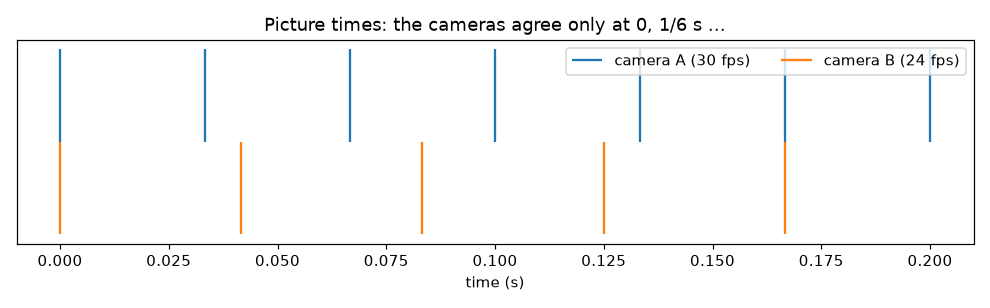
\includegraphics[width=0.85\linewidth]{figures/s01_two_clocks.png}\\\small Picture times of the two cameras: they agree only every 1/6 s.\end{center}

\subsection*{E. Worked example}
Camera B is turned 40 degrees. A square on the sheet is 100 pixels wide in camera A (looking straight on). How wide does it look sideways in a picture taken at the same scale by B? And how far does a sample moving at 120 px/s travel in the worst timing gap between a 30 fps and a 24 fps camera?
\begin{enumerate}[nosep]
\item Squeeze = cos 40 = 0.766.
\item Width in B at the same scale = 100 * 0.766 = 76.6 pixels.
\item Cameras agree every 1/gcd(30, 24) = 1/6 s. Within one cycle the A pictures are at 0, 1/30, 2/30, 3/30, 4/30 s and the B pictures at 0, 1/24, 2/24, 3/24 s.
\item The nearest-B distances for the five A pictures are 0, 8.33, 16.67, 16.67 and 8.33 ms. The worst gap is 16.7 ms = 1/60 s.
\item Distance moved = 120 px/s * (1/60) s = 2.0 px.
\end{enumerate}
\textbf{Answer.} The square looks 76.6 pixels wide, and the worst timing gap of 16.7 ms moves a 120 px/s sample by 2.0 px, which is a large error in a measurement that aims at hundredths of a pixel.

\subsection*{F. Questions}
\begin{enumerate}[nosep]
\item \textbf{Conceptual.} Why can one resize factor not bring camera B's picture onto camera A's picture in this set-up?
\item \textbf{Numerical.} A camera is turned 60 degrees to the side. A sideways distance is 100 pixels in a head-on picture. How long does it look? A sample at 90 px/s is paired with a picture 1/60 s away: how far has it moved?
\item \textbf{Graph and simulation interpretation.} In the timing graph (frame rate of B = 24), what is the highest the curve reaches, and what do the red dots tell you?
\item \textbf{Design and optimisation challenge.} Design: camera A runs at 30 fps. Which of these B frame rates keep the worst gap at or below 10 ms: 24, 25, 30, 48, 50, 60? Which would you choose, and what do you give up?
\end{enumerate}

\section{Session 2: One pixel grid and one time base}

\subsection*{A. Real-world problem}
Before any correlation, both cameras must give the same kind of data: the same pixel grid and the same clock. Camera B is 16:9 and sees the sample from the side; the sample is 4:3. Camera A samples the motion every 1/30 s and B every 1/24 s. How do you map B's picture onto a regular grid without wrecking the speckle? How do you fit a 16:9 picture into a 4:3 grid? And how do you put two series with different sample times on one timeline without inventing wiggles at a sudden jump? (A simplified educational model, not a validated measurement procedure.)

\subsection*{B. Concept and theory}
Geometry. A homography maps a flat sheet seen by one camera onto the same sheet seen by another: x' = (h11 x + h12 y + h13) / (h31 x + h32 y + 1), y' = (h21 x + h22 y + h23) / (h31 x + h32 y + 1). Multiplying out the denominator makes each point pair give two linear equations in the eight unknowns h, so four pairs give an 8 x 8 system. To build an output picture we use inverse mapping: for each output pixel find where it came from (H inverse) and read the source there with bilinear interpolation, a weighted average of the four neighbours. Aspect ratio. For a source of aspect r and a grid of aspect t, letterbox and crop both cost 1 - min(r, t) / max(r, t) of the pixels (empty grid pixels, or lost source pixels), while stretch costs nothing in pixels but scales y by max/min relative to x. Resampling. Bilinear sampling at a fractional position f weights two neighbours by (1 - f) and f, so white noise keeps sqrt((1-f)\textasciicircum{}2 + f\textasciicircum{}2) of its standard deviation: 0.707 at f = 0.5. Time. Both cameras are put on a 120 fps timeline (120 = 4 x 30 = 5 x 24). Makima builds a cubic Hermite curve through every sample. With segment slopes m\_i the slope at a sample is d\_i = (w1 m\_\{i-1\} + w2 m\_i) / (w1 + w2) with w1 = \textbar{}m\_\{i+1\} - m\_i\textbar{} + \textbar{}m\_\{i+1\} + m\_i\textbar{} / 2 and w2 = \textbar{}m\_\{i-1\} - m\_\{i-2\}\textbar{} + \textbar{}m\_\{i-1\} + m\_\{i-2\}\textbar{} / 2. The original Akima weights lack the second term and become 0/0 where neighbouring slopes agree; at a corner between a flat run and a ramp the fallback slope makes the curve dip below the data. Makima keeps the smaller slope there. It reproduces straight lines exactly, is not exact for quadratics (unlike Akima and the spline), is C1 (slope continuous) but not C2, and is local (a change in one sample reaches only a few intervals away) while the spline is global. Offset. If camera B's clock is late by tau, its picture labelled t shows the motion at t + tau; the lag that maximises the normalised cross-correlation of the two resampled series gives tau, refined by a parabola through the three points around the peak.

\begin{itemize}[nosep]
\item H: 3 x 3 homography matrix (h33 = 1) (no unit)
\item (x, y), (x', y'): pixel position before and after the map (pixels)
\item f: fractional part of a sampling position (pixels)
\item r, t: aspect ratio of the source picture and of the grid (no unit)
\item m\_i: slope of the straight segment from sample i to i+1 (px/s)
\item d\_i: Makima slope at sample i (px/s)
\item tau: timing offset of camera B (s)
\end{itemize}

\begin{equation*}
x'=\frac{h_{11}x+h_{12}y+h_{13}}{h_{31}x+h_{32}y+1},\qquad y'=\frac{h_{21}x+h_{22}y+h_{23}}{h_{31}x+h_{32}y+1}
\end{equation*}

\begin{equation*}
\begin{pmatrix}x&y&1&0&0&0&-xx'&-yx'\\0&0&0&x&y&1&-xy'&-yy'\end{pmatrix}\mathbf h=\begin{pmatrix}x'\\y'\end{pmatrix}
\end{equation*}

\begin{equation*}
\text{letterbox / crop cost}=1-\frac{\min(r,t)}{\max(r,t)},\qquad \text{stretch ratio}=\frac{\max(r,t)}{\min(r,t)}
\end{equation*}

\begin{equation*}
\frac{\sigma_{\text{after}}}{\sigma_{\text{before}}}=\sqrt{(1-f)^2+f^2}
\end{equation*}

\begin{equation*}
d_i=\frac{w_1m_{i-1}+w_2m_i}{w_1+w_2},\quad w_1=|m_{i+1}-m_i|+\tfrac12|m_{i+1}+m_i|,\quad w_2=|m_{i-1}-m_{i-2}|+\tfrac12|m_{i-1}+m_{i-2}|
\end{equation*}

\begin{equation*}
p(x)=h_{00}(t)y_i+h_{10}(t)\,\Delta x\,d_i+h_{01}(t)y_{i+1}+h_{11}(t)\,\Delta x\,d_{i+1},\qquad t=\frac{x-x_i}{\Delta x}
\end{equation*}

\begin{center}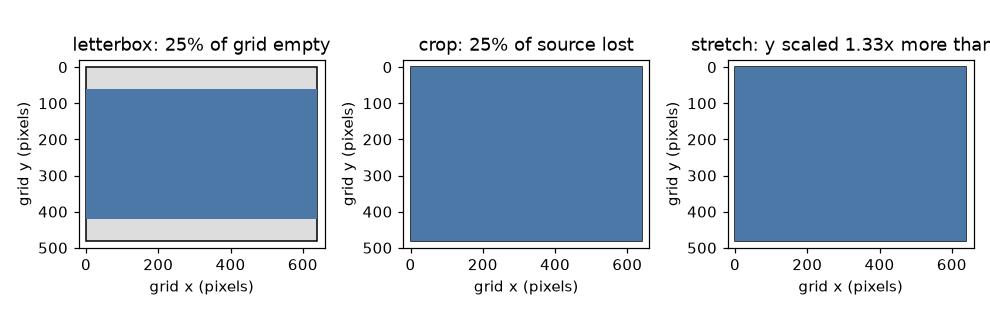
\includegraphics[width=0.85\linewidth]{figures/s02_aspect_fits.png}\\\small Letterbox, crop and stretch for a 16:9 picture in a 4:3 grid.\end{center}

\subsection*{E. Worked example}
A homography has H = [[1, 0.2, 10], [0, 1, 5], [0.001, 0, 1]]. Where does the pixel (100, 50) go, and does the inverse bring it back?
\begin{enumerate}[nosep]
\item Compute the denominator: w = 0.001 * 100 + 0 * 50 + 1 = 1.1.
\item Numerator for x: 1 * 100 + 0.2 * 50 + 10 = 120, so x' = 120 / 1.1 = 109.09.
\item Numerator for y: 0 * 100 + 1 * 50 + 5 = 55, so y' = 55 / 1.1 = 50.00.
\item The inverse matrix applied to (109.09, 50.00) returns (100, 50) (the checkpoint verifies this).
\end{enumerate}
\textbf{Answer.} The pixel (100, 50) goes to (109.09, 50.00), and the inverse brings it back to (100, 50).

\subsection*{F. Questions}
\begin{enumerate}[nosep]
\item \textbf{Conceptual.} Why do we build a warped picture by looking up, for each output pixel, where it came from, instead of moving each source pixel forward?
\item \textbf{Numerical.} Fit a 1280 x 720 camera picture into a 640 x 480 grid. How many rows of the grid stay empty with letterbox, and what fraction of the source is lost with crop?
\item \textbf{Graph and simulation interpretation.} In the interpolation figure, which curve overshoots the step, by how much, and why does RMS error alone not show this?
\item \textbf{Design and optimisation challenge.} Design: camera A is 4:3 and camera B is 16:9; the grid is 4:3 and you cannot afford to lose any of the sample's field of view, but the shape of speckle dots must stay round. Which fit do you choose? And which B frame rate (30 or 60) would you choose if you could?
\end{enumerate}

\section{Session 3: A mini stereo-DIC pipeline, validated against a known motion}

\subsection*{A. Real-world problem}
A flat speckled sample moves while camera A (4:3, 30 fps, almost head-on) and camera B (16:9, 24 fps, 28 degrees to the side) film it. We simulate the cameras, so the true motion is known exactly. Can the pipeline recover it to a fraction of a pixel? Which step matters most? And what happens when part of the sample leaves one camera's picture, or when you ask for data outside the time that was filmed? (A simplified educational model on synthetic data, not a validated measurement procedure.)

\subsection*{B. Concept and theory}
Each camera is a homography from the sheet to its picture, built from a focal length, a viewing angle and a distance. We click the four sheet corners in each picture (with a click error of 0.3 px) and solve a homography from the clicked camera pixels to the common 160 x 120 grid, where one grid pixel is one sheet unit. Each warped frame is compared with frame 0: a (2h+1) x (2h+1) subset, h = 10, is slid over every shift within +-6 px and scored by zero-normalised cross-correlation (ZNCC), which ignores brightness and contrast changes. The best whole-pixel shift is refined by a parabola through the peak and its neighbours: delta = (c\_- - c\_+) / (2 (c\_- - 2 c\_0 + c\_+)). Each camera's displacement series is resampled to the 120 fps timeline and the two are averaged. The truth is a motion amplitude s(t) with ux = s (1 + g (X - 80)), g = 0.004, and uy = 0.4 s. Error is the root-mean-square difference between merged data and truth over the nine subsets, both components and the timeline. We compare three geometries (homography, best affine fit, plain resize) and three timings (nearest sample, linear, Makima), and two correlation modes: against frame 0 (reference) or against the previous frame with the steps added up (consecutive).

\begin{itemize}[nosep]
\item s(t): true motion amplitude (px)
\item (ux, uy): true displacement of a subset (px)
\item h: subset half size (21 x 21 pixels) (px)
\item c(-1), c(0), c(+1): ZNCC scores around the best whole-pixel shift (no unit)
\item delta: sub-pixel correction from the parabola (px)
\item RMS: root-mean-square error against the truth (px)
\item g: gradient of the true displacement along x (1/px)
\end{itemize}

\begin{equation*}
\delta=\frac{c_{-}-c_{+}}{2\,(c_{-}-2c_{0}+c_{+})}
\end{equation*}

\begin{equation*}
\mathrm{ZNCC}=\frac{\sum (f-\bar f)(g-\bar g)}{\sqrt{\sum (f-\bar f)^2\,\sum (g-\bar g)^2}}
\end{equation*}

\begin{equation*}
u_x=s(t)\,\big(1+g\,(X-80)\big),\qquad u_y=0.4\,s(t)
\end{equation*}

\begin{equation*}
\mathrm{RMS}=\sqrt{\frac{1}{N}\sum\big(u_{\mathrm{merged}}-u_{\mathrm{true}}\big)^2}
\end{equation*}

\begin{center}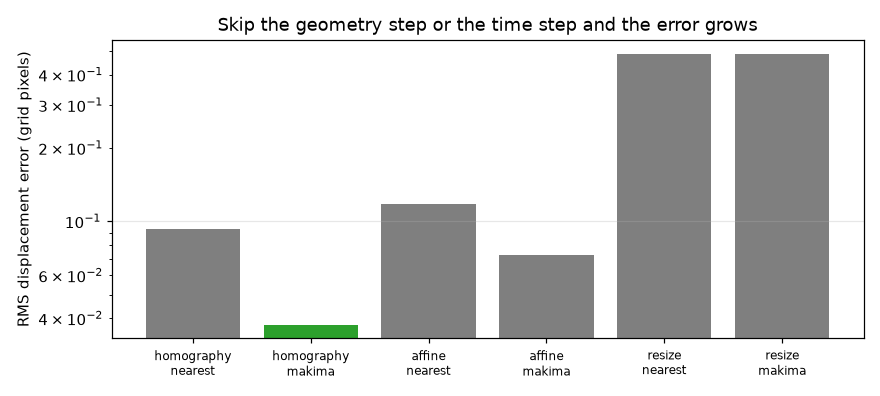
\includegraphics[width=0.85\linewidth]{figures/s03_error_budget.png}\\\small Merged RMS error for six geometry and timing choices on a step-like motion (logarithmic axis).\end{center}

\subsection*{E. Worked example}
A subset's ZNCC scores at whole-pixel shifts 2, 3 and 4 are 0.80, 0.95 and 0.90. What sub-pixel shift does the parabola give? And is the pipeline's whole recipe, camera model plus homography, consistent for the synthetic pair?
\begin{enumerate}[nosep]
\item The best whole-pixel shift is 3 (score 0.95); its neighbours are c(-1) = 0.80 and c(+1) = 0.90.
\item delta = (0.80 - 0.90) / (2 * (0.80 - 2 * 0.95 + 0.90)) = (-0.10) / (2 * (-0.20)) = 0.25.
\item The shift is 3 + 0.25 = 3.25 px.
\item For the synthetic pair, warping picture B onto A's pixel grid with the homography solved from the four sheet corners gives a correlation with A above 0.99 (the checkpoint prints 0.999).
\end{enumerate}
\textbf{Answer.} The sub-pixel shift is 3.25 px, and the warped synthetic picture B matches picture A with a correlation of 0.999.

\subsection*{F. Questions}
\begin{enumerate}[nosep]
\item \textbf{Conceptual.} Why does correlating each frame with the previous frame and adding up the steps give a larger error than correlating each frame with frame 0?
\item \textbf{Numerical.} ZNCC scores 0.60, 0.90 and 0.85 at shifts 4, 5 and 6. Find the sub-pixel shift. Give the unit.
\item \textbf{Graph and simulation interpretation.} In the error-budget bar chart (step-like motion), read the five errors: homography with Makima, homography with nearest, affine with Makima, and resize with nearest. What does each bar tell you to fix first?
\item \textbf{Design and optimisation challenge.} Design: part of the sample leaves camera B's picture, so 3 of the 9 subsets cannot be measured in B. What do you do with the missing pixels, and what do you do about times where only one camera has data? Justify with the numbers.
\end{enumerate}

\section{Real-world mini-project}
\textbf{Align a 30 fps 4:3 camera and a 24 fps 16:9 camera, and report the error before and after.} Two cameras film a speckled sample that jumps like a step. Camera A is 240 x 180 (4:3) at 30 fps, camera B is 320 x 180 (16:9) at 24 fps and looks 28 degrees to the side. Use \texttt{before\_after('step')} and \texttt{run\_pipeline} from Session 3 to measure the displacement error with no alignment (pictures only resized to the grid, frames paired by nearest time) and with alignment (homography and Makima). Optional: drop your own view\_a.png and view\_b.png (and points.txt) into a folder named data next to start.py, run Session 3, and look at the picture pair\_on\_grid.png it saves.

\section{The path ahead}
\begin{enumerate}[nosep]
\item \textbf{Session 4: Lens distortion.} A distortion model (one radial term) fitted from the sheet corners and edge points, applied before warping.
\item \textbf{Session 5: Calibration targets and 3-D triangulation.} A calibration routine plus triangulation of matched points into millimetres.
\item \textbf{Session 6: Rolling-shutter correction.} A simulator with a row-by-row readout and a correction that resamples each row in time.
\item \textbf{Session 7: Correlation at GPU speed.} A batched correlator that handles a 100 x 100 grid of subsets per frame pair.
\item \textbf{Session 8: Your own cameras.} A run of Session 3 on your own two videos, with points.txt, an estimated offset and a written error budget.
\end{enumerate}

\section{Answers and hints}

\subsection*{Session 1}
\begin{enumerate}[nosep]
\item \textbf{Conceptual.} Hint: Compute the sideways and the up-down stretch from the sheet corners and compare them. Solution: The sideways stretch is 40 / (60 cos 40) = 0.870 and the up-down stretch is 40 / 60 = 0.667. They differ because B is turned (its sideways distances are squeezed by cos 40) and the pictures have different scales. A single resize factor can only apply one number, so a transform with different sideways and up-down parts (and, in general, perspective, which is Session 2) is needed.
\item \textbf{Numerical.} Hint: Use squeeze = cos(yaw) and distance = speed * gap. Solution: cos 60 = 0.5, so the distance looks 100 * 0.5 = 50 pixels (units: pixels). The sample moves 90 * (1/60) = 1.5 px. Sanity check: at 90 degrees the squeeze would be 0, the sheet seen edge-on, which is why very large angles are useless.
\item \textbf{Graph and simulation interpretation.} Hint: The curve is the distance to the nearest B picture; the dots are read at the A picture times. Solution: The curve reaches half a B period, 1/48 s = 20.8 ms, in the middle between two B pictures. The red dots at the A picture times read 0, 8.33, 16.67, 16.67 and 8.33 ms over one 1/6 s cycle, so the worst gap seen by any A picture is 16.7 ms, below the curve's peak because A pictures do not fall exactly in the middle of a B interval.
\item \textbf{Design and optimisation challenge.} Hint: Use the timing view or worst\_gap(30, fps) in lesson.py. Solution: The worst gaps are 16.7 ms (24), 20 ms (25), 0 (30), 8.3 ms (48), 6.7 ms (50) and 0 (60). So 30, 48, 50 and 60 are within 10 ms. 30 or 60 give exact agreement (gap 0) but only if the two clocks start together; 60 doubles the data and needs more light and storage. Trade-off: a perfectly matched pair removes the need for time interpolation, but you often cannot choose, so Session 2 shows how to interpolate instead.
\end{enumerate}

\subsection*{Session 2}
\begin{enumerate}[nosep]
\item \textbf{Conceptual.} Hint: What happens to output pixels that no source pixel lands on? Solution: Pushing source pixels forward leaves holes in the output (some output pixels get no source pixel) and collisions (some get several). Inverse mapping visits every output pixel exactly once and asks where it came from, so every output pixel gets a value. The source position is usually between pixels, so we read it with bilinear interpolation.
\item \textbf{Numerical.} Hint: Scale = 640 / 1280 = 0.5 shrinks the picture to 640 x 360. Solution: Letterbox: the picture becomes 640 x 360, so 480 - 360 = 120 grid rows are empty, 60 above and 60 below: 120 / 480 = 25 percent. Crop: scale by 480 / 720 = 0.667 to 853 x 480 and keep 640 of the 853 columns, losing 213 / 853 = 25 percent. Stretch keeps everything but scales y by 0.667 / 0.5 = 1.33 relative to x.
\item \textbf{Graph and simulation interpretation.} Hint: Compare the highest value of each curve with the top of the step, 4 px. Solution: The cubic spline overshoots by about 0.38 px at 24 fps; linear and Makima stay between 0 and 4 px. The spline is smooth everywhere, so near a jump it must swing past the data to keep its curvature continuous. RMS averages over the whole window, so a short overshoot can hide inside a similar number; the step-like RMS errors are Makima 0.055, linear 0.123 and spline 0.147 px, and the spline is worst even though it is the best method on smooth motion (0.0014 px against Makima 0.0083 and linear 0.0394).
\item \textbf{Design and optimisation challenge.} Hint: Compare the three costs for 16:9 into 4:3 and recall the gaps for 30 and 60 fps. Solution: Crop loses 25 percent of the field of view, so it is out. Stretch keeps the field of view but makes dots elliptical (1.33 : 1). Letterbox keeps both field of view and round dots at the price of 25 percent empty grid, which is acceptable if the sample fits in the central 75 percent of the height. Frame rate: at 30 or 60 fps the picture times agree with A exactly (gap 0) if the clocks start together; 60 fps also gives the smaller step-like error, about 0.036 px for Makima in the app, but doubles the data.
\end{enumerate}

\subsection*{Session 3}
\begin{enumerate}[nosep]
\item \textbf{Conceptual.} Hint: Each step has a small error; think about what happens when you add 23 of them. Solution: Every step carries a small error (the parabola bias and noise). Adding steps adds their errors, which grows with the number of frames (a random-walk drift), while correlating with frame 0 gives each frame its own independent error. In the simulation the merged RMS is 0.083 px with consecutive correlation against 0.023 px with the reference frame. The reference method needs a search window large enough for the whole motion, which is why consecutive correlation is used for large motions.
\item \textbf{Numerical.} Hint: Use delta = (c(-1) - c(+1)) / (2 (c(-1) - 2 c(0) + c(+1))) around the best whole shift 5. Solution: delta = (0.60 - 0.85) / (2 * (0.60 - 1.80 + 0.85)) = (-0.25) / (2 * (-0.35)) = 0.357. The shift is 5.357 px. Sanity check: the right neighbour (0.85) is higher than the left one (0.60), so the true peak lies to the right of 5, and delta is between 0 and 0.5 as it must be.
\item \textbf{Graph and simulation interpretation.} Hint: Compare each bar with the lowest one. Solution: Homography with Makima is the lowest at 0.038 px. Pairing frames by nearest time instead raises it to 0.093 px (2.4 times). Using an affine fit instead of the homography raises it to 0.073 px (1.9 times), almost entirely from camera B, whose perspective an affine map cannot describe. A plain resize with nearest pairing gives 0.485 px (13 times), because the two cameras then measure in different pixel units. Fix the geometry first (it has the largest effect), then the timing.
\item \textbf{Design and optimisation challenge.} Hint: Compare masking the missing pixels with filling them with zeros, and check what the merge does at the end of a camera's time range. Solution: Mask them: a subset that touches missing pixels returns NaN and the merge uses camera A alone there. The merged RMS stays at 0.024 px, against 0.053 px if the missing pixels are filled with zeros (the black edge is static and pulls the subset towards zero displacement). For time, never extrapolate by default: continuing Makima beyond the last sample gives errors of 0.39, 2.31 and 7.04 px one, two and three frames beyond the end, against 0.009 px inside the range. Use the other camera, or stop the data where both have samples.
\end{enumerate}

\section{How to join}
Read \texttt{CONTRIBUTING.md} in the repository, then pick an issue labelled \texttt{good first issue}. Repository: \url{https://github.com/KrunalPanchal1995/openstitchdic}

\end{document}
